\documentclass{beamer}
\title{Archeologia podwodna}
\author{Klaudia Rutkowska}
\date{\today}
\institute{UWM}
\usepackage{amsfonts}
\usepackage{graphicx}
\usepackage[MeX]{polski}
\begin{document}
\frame{\titlepage}
%\begin{frame}
%\frametitle{Spis treści}
%\tableofcontents
%\end{frame}

\section{Wstęp}

\begin{frame}{Archeologia podwodna}
Archeologia podwodna, prospekcja podwodna jest odłamem archeologii, który wyodrębniony został na podstawie wykorzystywanych metod badawczych i środowiska badawczego.
\end{frame}

\begin{frame}{Archeologia podwodna -cd.}
\begin{center}
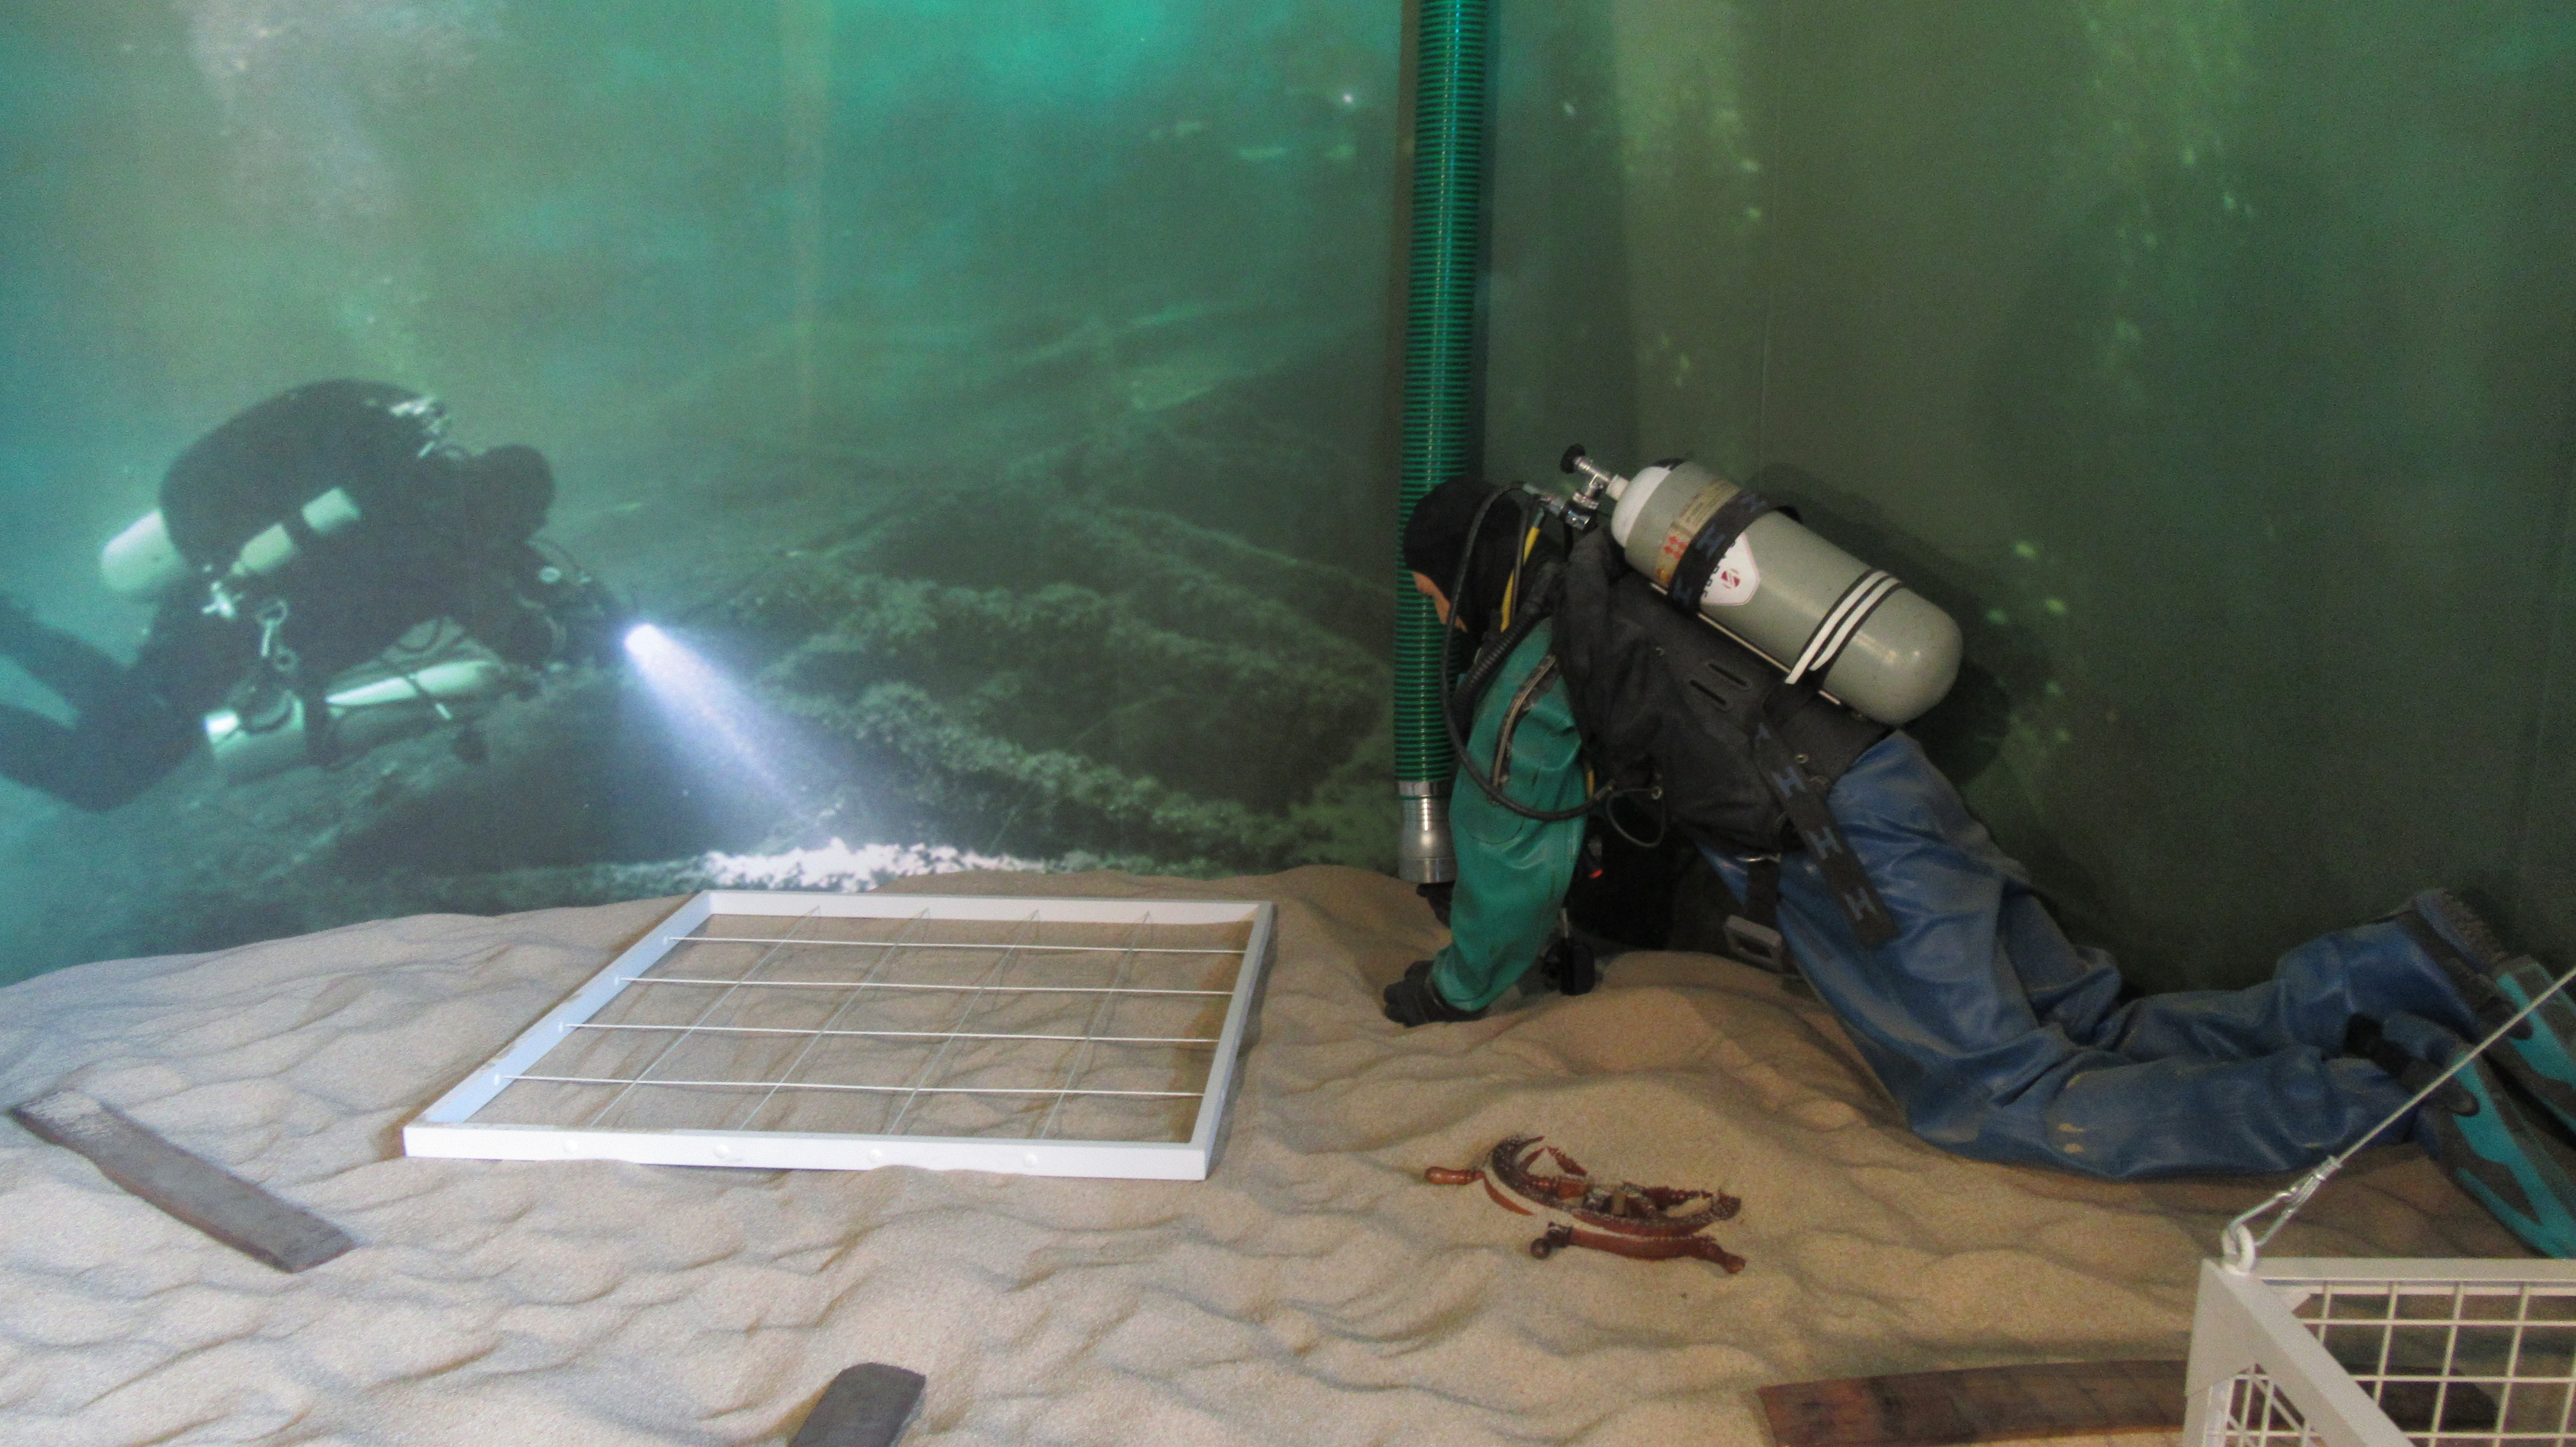
\includegraphics[width=8cm]{mumin.jpg}
\label{mumin.jpg}
\end{center}
\end{frame}

\begin{frame}{Wstęp}
Początków tej gałęzi nauki należy się dopatrywać na przełomie lat 1853-1854, kiedy to po raz pierwszy w Zurychu zetknięto się z dużą ilością artefaktów, odsłoniętych na skutek obniżającego się poziomu wód w jeziorach.

Podobnie jak ma to miejsce na lądzie, badania prospekcyjne zmierzają do lokalizacji nowych i szczegółowego rozpoznania znanych już stanowisk. Stanowiska archeologii podwodnej poszukuje się we wszelkiego rodzaju zbiornikach wodnych od jezior, źródeł i rzek, poprzez zatopione studnie, miasta, porty, aż do zalanych jaskiń, a nade wszystko morza i oceany oraz związane z tym, wraki statków. Ze względu na duże zainteresowanie archeologów dwoma ostatnimi rodzajami zbiorników, archeologia podwodna często określana jest jako archeologia morska.
\end{frame}

\section{Kwerenda}
\begin{frame}{Kwerenda}
Przed pracami podwodnymi badacze zapoznają się z danymi źródłowymi. Studiowanie map, dzienników i dokumentów naprowadza badaczy na zatopiony okręt lub port. Wywiady przeprowadzane z miejscową ludnością okazują się źródłem wielu cennych informacji (poławiacze pereł czy też gąbek spędzają wiele godzin pod wodą i mogą naprowadzić badaczy na trop okrętu lub ruin).
\end{frame}

\section{Rozpoznanie}
\begin{frame}{Rozpoznanie}
Pod wodą możliwe jest prowadzenie odpowiednika badań powierzchniowych. Zespół nurków wyposażonych w płetwy i aparaty do nurkowania przeszukuje w tyralierze wyznaczony obszar, rejestrując i lokalizując stanowiska archeologiczne.

Do rozpoznania podwodnego w archeologii wykorzystuje się również metody geofizyczne. Łodzie mogą holować podwieszony w odpowiedniej odległości magnetometr, który wykrywa przedmioty wykonane ze stali i żelaza. Nadajnik sonaru może emitować ultradźwięki, których odbicie po zarejestrowaniu jest przetwarzane w graficzny obraz ukształtowania dna. Dzięki umieszczonemu pod łodzią sonarowi poddennemu możliwe jest uzyskanie obrazu obiektów ukrytych pod dnem.

Archeologia lotnicza także ma swój udział w badaniach podwodnych. Obiekty znajdujące się na niewielkiej głębokości są doskonale widoczne z powietrza w słoneczny dzień, jeśli woda nie jest mętna.
\end{frame}


\begin{frame}{Prowadzenie wykopalisk}
\section{Prowadzenie wykopalisk}
Wykopaliska podwodne są trudne do przeprowadzenia, skomplikowane i kosztowne. Wymagają także natychmiastowej konserwacji wydobywanych na powierzchnię przedmiotów. Badania takie polegają na przemieszczaniu dużej ilości osadów i dokumentowaniu oraz wydobywaniu na powierzchnię dużych obiektów, takich jak naczynia zasobowe, amfory, sztaby żelaza, złota czy też armaty.

Archeologia podwodna wykorzystuje zróżnicowane narzędzia, które znacznie rozwijały się na przestrzeni wieków. Do ważniejszych zaliczamy sprzęt do nurkowania (skafandry, butle, automaty oddechowe itp.), zdalnie sterowane roboty podwodne, miniaturowe łodzie podwodne, które umożliwiają zejście w głąb mórz i oceanów, gdzie granica ludzkiej wytrzymałości została naruszona, różnego rodzaju kosze na znaleziska. Rejestruje się obraz za pomocą kamer i aparatów, przystosowanych do prac podwodnych.

W trakcie badań sami archeolodzy wynaleźli urządzenia pomocne w podwodnych pracach. Za przykład można podać balon umocowany do koszyka, który ułatwia wydobywanie zabytków na powierzchnię.

Jeśli odkryto zachowany kadłub, wykonuje się jego szczegółowy rysunek, który umożliwi w przyszłości jego rekonstrukcję po wydobyciu na powierzchnię.
\end{frame}

\begin{frame}{Podsumowanie}
Działalność archeologii podwodnej przejawia się przede wszystkim w dokumentowaniu i wyławianiu zachowanych przedmiotów z dna zbiorników, śladów dawnej ludzkiej działalności.

Archeolodzy podwodni na podstawie swoich badań dokonali szeregu analiz, które pozwoliły poznać nie tylko konstrukcje zatopionych statków i obiektów, ale także poznać szczegóły życia na statkach. Ustalono rodzaje przewożonych towarów, poznano m.in. dawną metalurgię i produkcję szkła, odkrywając niepowtarzalne zabytki.
\end{frame}

\end{document}
